\documentclass[a4paper,10pt]{article}

\usepackage[brazilian]{babel}
\usepackage[utf8]{inputenc}
\usepackage[T1]{fontenc}
\usepackage{titlesec}
\usepackage{graphicx}
\usepackage{mathtools}
\usepackage{amsthm}
\usepackage[top=1.0in,bottom=1.0in]{geometry}
\usepackage{hyperref}
\usepackage[singlelinecheck=false]{caption}
\usepackage[backend=biber,url=true,doi=true,eprint=false]{biblatex}

\addbibresource{../common/references.bib}

\newcommand\blfootnote[1]{%
  \begingroup
  \renewcommand\thefootnote{}\footnote{#1}%
  \addtocounter{footnote}{-1}%
  \endgroup
}

\newcommand\defeq{\mathrel{\overset{\makebox[0pt]{\mbox{\normalfont\tiny\sffamily def}}}{=}}}

\titleformat{\section}
  {\normalfont\scshape\bfseries}{\thesection}{1em}{}
\titleformat{\subsection}
  {\normalfont\scshape\bfseries}{\thesubsection}{1em}{}
\titleformat{\paragraph}
  {\normalfont}{\theparagraph}{1em}{}
\titleformat{\subparagraph}
  {\normalfont}{\thesubparagraph}{1em}{}

\captionsetup[table]{labelsep=space}

\theoremstyle{plain}

\newtheorem*{spn-def}{Definição}
\newtheorem*{spn-thm}{Teorema}

\title{\textbf{Modeling and Reasoning with Bayesian Networks: Compiling Bayesian Networks}}

\begin{document}
\date{}
\author{}
\vspace*{-40pt}
{\let\newpage\relax\maketitle}

Relatório semana 1 - MAC0215 (Atividade Curricular em Pesquisa)

Aluno: Renato Lui Geh (Bacharelado em Ciência da Computação)

Orientador: Denis Deratani Mauá

\section{Atividades realizadas na semana}

\paragraph{
  Durante a semana foram lidos os seguintes tópicos do livro \textit{Modeling and Reasoning with
Bayesian Networks}\cite{bayes-net-darwiche}:
}

\begin{description}
  \item[12] - Compiling Bayesian Networks
  \begin{description}
    \item[12.1] - Introduction
    \item[12.2] - Circuit semantics
    \item[12.3] - Circuit propagation
    \begin{description}
      \item[12.3.1] - Evaluation and differentiation passes
    \end{description}
  \end{description}
\end{description}

\section{Definição das atividades}

\paragraph{
  Foram estudados o processo de se compilar Redes Bayesianas em circuitos aritméticos, algumas
notações usadas em Redes Bayesianas, a definição de uma \textit{network polynomial}, algumas
propriedades de Redes Bayesianas e diferenciação de uma rede a partir de uma evidência.
}

\paragraph{
  Esta seção será dividida em subseções para cada subtópico citado na seção anterior. Cada
subseção é um resumo do que foi estudado em cada tópico, contendo os assuntos mais importantes
para o projeto.
}

\subsection{Introduction}

\paragraph{
  Aqui apresentaremos algumas notações usadas em Redes Bayesianas - e que podem ser extendidas para
outros Modelos Gráficos Probabilísticos (PGM).
}

\begin{figure}[h]
\centering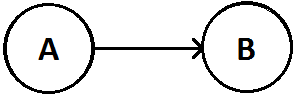
\includegraphics[scale=0.5]{imgs/fig1.png}
\caption{Uma Rede Bayesiana $A \to B$. Em Redes Bayesianas uma aresta representa uma dependência.
  No caso da imagem $B$ depende de $A$. As CPTs associadas a esse grafo estão em Tabela 1 e
  Tabela 2.}
\end{figure}

\begin{table}[h]
\begin{center}
\captionsetup{justification=centering}
\caption{ e Tabela 2}
\begin{tabular}{c | c}
  A  & $\Theta_A$ \\
\hline
true & $\theta_a = 0.3$ \\
false& $\theta_{\overline{a}} = 0.7$ \\
\end{tabular}
\quad
\quad
\begin{tabular}{c c | c}
A & B & $\Theta_{B|A}$ \\
\hline
true & true & $\theta_{b|a} = 0.1$ \\
true & false & $\theta_{\overline{b}|a} = 0.9$ \\
false & true & $\theta_{b|\overline{a}} = 0.8$ \\
false & false & $\theta_{\overline{b}|\overline{a}} = 0.2$ \\
\end{tabular}
\end{center}
\end{table}

\paragraph{
  Antes de começarmos com circuitos aritméticos, vamos primeiro apresentar algumas definições
importantes.
}

\paragraph{
  Chamamos de CPT (Conditional Probability Table) as tabelas que representam as
probabilidades de uma rede (ex.: as CPTs da Rede Bayesiana na Figura 1 são as Tabelas 1 e 2).
Pode-se claramente ver que para $n$ nós de uma Rede Bayesiana, precisamos de uma quantidade
exponencial $2^n$ de probabilidades para representar cada instância de variáveis.
}

\paragraph{
  Chamamos de MPE (Most Probable Explanation) a instância mais provável de variáveis que aceitam
uma evidência. Mais formalmente dizemos que:
}

\begin{spn-def} Sejam $X_1,...,X_n$ as variáveis da rede e $e$ a evidência dada. Existe uma
  instância $x_1,...,x_n$ onde $Pr(x_1,...,x_n|e)$ é maximal. Chamamos $x_1,...,x_n$ a
  \textit{explicação mais provável} (\textit{most probable explanation}) dado $e$.
\end{spn-def}

\paragraph{
  Chamamos de MAP (Maximum A Posteriori hypothesis) quando a probabilidade de uma certa instância
é maximal.
}

\begin{spn-def} Sejam $X$ o conjunto de todas as variáveis da rede e $M$ um subconjunto qualquer
  dessas variáveis. Dado uma evidência $e$, qualquer instância $m$ de variáveis $M$ onde $Pr(m|e)$
  é maximal é uma \textit{hipótese máxima a posteriori} (\textit{maximum a posteriori hypothesis}).
\end{spn-def}

\paragraph{
  $M$ também é chamado de variáveis MAP. MPE é uma MAP quando as variáveis MAP incluem todas as
variáveis da rede.
}

\paragraph{
  Agora que temos uma base podemos voltar para circuitos aritméticos. Dado um circuito aritmético
que representa uma Rede Bayesiana, teremos dois tipos de entradas: variáveis $\theta$, que
chamaremos de \textit{parâmetros}, e as variáveis $\lambda$, que chamaremos de
\textit{indicadores}. Parâmetros são valorados de acordo com a CPT da rede, enquanto indicadores
são valorados de acordo com a evidência. Nas próximas subseções veremos que podemos ter duas
passagens pelo circuito. Uma em que vamos de baixo para cima (bottom-up) para calcular a
probabilidade de uma dada evidência, e outra em que vamos de cima para baixo (top-down), chamada
de \textit{differentiation pass} para calcularmos as derivadas parciais de cada entrada do
circuito.
}

\subsection{Circuit semantics}

\paragraph{
  Ao compilarmos um circuito aritmético de uma Rede Bayesiana estamos representando, de forma
compacta, a distribuição de probabilidade induzida da rede. No caso da Figura 1, a distribuição de
probabilidade está representada na Tabela 3.
}

\setcounter{table}{2}

\begin{table}[h]
\begin{center}
\captionsetup{justification=centering}
\caption{}
\begin{tabular}{c c | c}
$A$ & $B$ & $Pr(A, B)$ \\
\hline
$a$ & $b$ & $\theta_{a}\theta_{b|a}$ \\
$a$ & $\overline{b}$ & $\theta_{a}\theta_{\overline{b}|a}$ \\
$\overline{a}$ & $b$ & $\theta_{\overline{a}}\theta_{b|\overline{a}}$ \\
$\overline{a}$ & $\overline{b}$ & $\theta_{\overline{a}}\theta_{\overline{b}|\overline{a}}$ \\
\end{tabular}
\end{center}
\end{table}

\newpage

\paragraph{
  Multiplicando cada $Pr(A, B)$ com as suas respectivas variáveis indicadoras temos que:
}

\begin{table}[h]
\begin{center}
\captionsetup{justification=centering}
\caption{}
\begin{tabular}{c c | c}
$A$ & $B$ & $Pr(A, B)$ \\
\hline
$a$ & $b$ & $\lambda_{a}\lambda_{b}\theta_{a}\theta_{b|a}$ \\
$a$ & $\overline{b}$ & $\lambda_{a}\lambda_{\overline{b}}\theta_{a}\theta_{\overline{b}|a}$ \\
$\overline{a}$ & $b$ & $\lambda_{\overline{a}}\lambda_{b}\theta_{\overline{a}}\theta_{b|\overline{a}}$ \\
$\overline{a}$ & $\overline{b}$ & $\lambda_{\overline{a}}\lambda_{\overline{b}}\theta_{\overline{a}}\theta_{\overline{b}|\overline{a}}$ \\
\end{tabular}
\end{center}
\end{table}

\paragraph{
  Somando todas as probabilidades da distribuição temos:
}

\begin{equation}
f = \lambda_{a}\lambda_{b}\theta_{a}\theta_{b|a} +
  \lambda_{a}\lambda_{\overline{b}}\theta_{a}\theta_{\overline{b}|a} +
  \lambda_{\overline{a}}\lambda_{b}\theta_{\overline{a}}\theta_{b|\overline{a}} +
  \lambda_{\overline{a}}\lambda_{\overline{b}}\theta_{\overline{a}}\theta_{\overline{b}|\overline{a}}
\end{equation}

\paragraph{
  Chamamos a função $f$ de \textit{network polynomial}, que representa a distribuição de
probabilidade da rede na Figura 1. Para computar a probabilidade dada qualquer evidência $e$,
definimos cada variável indicadora de forma consistente com a evidência. Vamos definir o que
significa definir uma variável de forma consistente com uma evidência:
}

\begin{spn-def} Sejam um conjunto $X=\{x_1,...,x_n,\overline{x}_1,...,\overline{x}_n\}$ das
variáveis da rede e uma evidência $e=\{e_p,...,e_q\}$. Dizemos que $X$ está consistente com $e$
quando para cada $e_i$, se $e_i=1$ então $x_i=1$ e $\overline{x}_i=0$; e se $e_i=0$ então $x_i=0$
e $\overline{x}_i=1$. Para todo $j$ tal que $1\leq{j}\leq{n}$ e que não exista um $e_j \in e$
definiremos $x_j=\overline{x}_j=1$. Por questões de visibilidade, definimos $(x_i, \overline{x}_i)$
ao invés de $(\lambda_{i}, \lambda_{\overline{i}})$, porém as notações são equivalentes.
\end{spn-def}

\paragraph{
  Portanto, se por exemplo tivermos evidência $e=\overline{a}$, teremos na \textit{network
polynomial} da Figura 1 os seguintes indicadores: $\lambda_{a}=0, \lambda_{\overline{a}}=1,
\lambda_{b}=1, \lambda_{\overline{b}}=1$. Neste exemplo, o valor de $f$ seria:
}

\begin{equation}
\begin{split}
f(\textbf{e}=\overline{a}) & = (0)(1)\theta_{a}\theta_{b|a} + (0)(1)\theta_{a}\theta_{\overline{b}|a} +
  (1)(1)\theta_{\overline{a}}\theta_{b|\overline{a}} +
  (1)(1)\theta_{\overline{a}}\theta_{\overline{b}|\overline{a}} \\
& = \theta_{\overline{a}}\theta_{b|\overline{a}} + \theta_{\overline{a}}\theta_{\overline{b}|\overline{a}} \\
& = Pr(\textbf{e})
\end{split}
\end{equation}

\paragraph{
  Como a \textit{network polynomial} de uma rede é a distribuição de probabilidade da rede, então
seu tamanho é exponencial. O circuito aritmético é uma representação compacta de $f$. Em alguns
casos $f$ não pode ser limitado, enquanto que o circuito pode.
}

\paragraph{
  Vamos definir formalmente uma \textit{network polynomial}, mas antes vamos definir algumas
notações. Dizemos que $\theta_{x|\textbf{u}} \sim \textbf{z}$ para dizer que $x\textbf{u}$ é
consistente com $\textbf{z}, x\textbf{u} \sim \textbf{z}$. Portanto,
$\prod_{\theta_{x|\textbf{u}} \sim \textbf{z}} \theta_{x|\textbf{u}}$ denota o produto de todos
os parâmetros $\theta_{x|\textbf{u}}$ onde $x\textbf{u}$ seja consistente com $\textbf{z}$. A mesma
notação aplica-se a $\lambda_x \sim \textbf{z}$.
}

\begin{spn-def} Seja $\mathcal{N}$ uma Rede Bayesiana sob variáveis $\mathbf{Z}$. Para cada
variável $X$ com pais $\mathbf{U}$, chamamos de $\lambda_x$ o indicador de $x$ e
$\theta_{x|\textbf{u}}$ o parâmetro. A \textit{network polynomial} de $\mathcal{N}$ é definida como:
\begin{equation}
f \defeq \sum_x \prod_{\theta_{x|\textbf{u}} \sim \textbf{z}} \theta_{x|\textbf{u}} \prod_{\lambda_x \sim \textbf{z}} \lambda_x.
\end{equation}
O valor da \textit{network polynomial} $f$ com evidência $e$ é o resultado da função $f(e)$
substituindo cada indicador $\lambda_x$ em $f$ com um valor consistente com $e$.
\end{spn-def}

\begin{spn-thm} Sejam $\mathcal{N}$ uma Rede Bayesiana, $Pr$ a distribuição de probabilidade
induzida e $f$ a \textit{polynomial}. Para toda evidência $e$, temos que $f(e)=Pr(e)$.
\end{spn-thm}

\subsection{Circuit propagation}

\paragraph{
  Nesta subseção definiremos o que são derivadas parciais e sua utilidade em Redes Bayesianas.
}

\paragraph{
  A derivada parcial de uma variável representa o quanto a mudança de uma variável impacta na saída
final da rede. Portanto, seja $\lambda_{\overline{a}}=0$ e sua derivada parcial
$\partial{f}/\partial{\lambda_{\overline{a}}} = 0.4$, e dada evidência $e=a\overline{c}$ e seja o
valor final de $f(e)=0.1$, ao mudarmos o valor de $\lambda_{\overline{a}}=1$, estaremos na realidade
mudando a evidência de $a\overline{c}$ para $\overline{c}$, e portanto teremos um valor final de
0.5 ao invés de 0.1, que representa justamente $f(\overline{c})$. Como pode-se notar, ter a
derivada parcial evita termos de computar toda vez a rede, já que temos as diferenças no próprio
circuito.
}

\paragraph{
  Vamos definir uma notação de mudança de evidência. Sejam uma evidência $e$ e $X$ um conjunto
de variáveis. Dizemos que $e-X$ é todos os elementos de $e$ menos aqueles que são equivalentes a
qualquer elemento do conjunto $X$. Por exemplo, se $e=ab\overline{c}$, então $e-A=b\overline{c}$
e $e-AC=b$.
}

\begin{spn-thm} Sejam $\mathcal{N}$ uma Rede Bayesiana, $Pr$ a distribuição de probabilidade, $f$ a
\textit{network polynomial} e $\textbf{e}$ uma evidência qualquer. Para cada indicador $\lambda_x$
temos que:
\begin{equation}
\frac{\partial{f}}{\partial{\lambda_x}}(\textbf{e}) = Pr(x, \textbf{e} - X)
\end{equation}
Além disso, para cada parâmetro $\theta_{x|\textbf{u}}$ temos que:
\begin{equation}
\theta_{x|\textbf{u}}\frac{\partial{f}}{\partial{\theta_{x|\textbf{u}}}}(\textbf{e})=Pr(x,\textbf{u},\textbf{e})
\end{equation}
Disso chega-se diretamente que:
\begin{equation}
\frac{\partial{f}}{\partial{\theta_{x|\textbf{u}}}}(\textbf{e})=\frac{Pr(x,\textbf{u},\textbf{e})}{\theta_{x|\textbf{u}}},
\qquad \text{quando $\theta_{x|\textbf{u}} \neq 0$.}
\end{equation}
Essa derivada é mais comumente escrita como:
\begin{equation}
\frac{\partial{f}}{\partial{\theta_{x|\textbf{u}}}}(\textbf{e})=\frac{\partial{Pr(\textbf{e})}}{\partial{\theta_{x|\textbf{u}}}},
\qquad \text{onde $Pr$ é a distribuição de $f$.}
\end{equation}
\end{spn-thm}

\subsection{Evaluation and differentiation passes}

\paragraph{
  Na subseção 12.3.1 do livro vimos como implementar as passagens \textit{top-down} e
\textit{bottom-up}. Em seguida analisamos a complexidade das duas passagens. Não vamos citar os
algoritmos neste relatório pois não é de muita importância para o projeto. No entanto, é
interessante citar as complexidades dos algoritmos.
}

\paragraph{
  No algoritmo de \textit{bottom-up}, a complexidade em tempo foi linear ao tamanho do circuito,
onde o tamanho foi definido como o número de arestas no circuito.
}

\paragraph{
  No algoritmo de \textit{top-down}, a princípio o algoritmo era linear se o número de nós crianças
era limitado. Porém, no segundo algoritmo garantimos que fosse linear sempre, já que se um nó era
zero, não guardávamos os nós crianças dele.
}

\section{Conclusão}

\paragraph{
  Estudou-se algumas notações em Redes Bayesianas que são indispensáveis para aprender Sum-Product
Networks. Além disso, o estudo de \textit{network polynomial}, que é bastante presente em PGMs é
um requerimento importante para SPNs. Também adquiriu-se uma noção básica de circuitos
aritméticos e de como implementa-los. Um outro ponto importante foi diferenciação parcial de
variáveis, que evita termos de passar várias vezes pelo circuito quando mudamos a evidência.
}

\newpage

\printbibliography

\end{document}
